\begin{figure}[t]
\centering
% Vector drawing generated by tools/figures/relbench_cumulative.py from exp/2026-10-20-relbench/paper-sessions.json; rerun it after the numbers change.
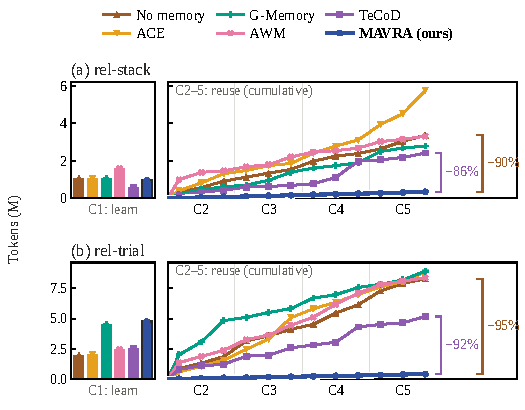
\includegraphics[width=\linewidth]{figures/relbench-cumulative}%
\caption{\bt{Tokens with memory operations: learning at cutoff 1 (bars) and cumulative reuse over cutoffs 2--5 (lines). Brackets give \system{}'s reuse-stage saving.}{含记忆操作的 token：截点 1 的学习（柱）与截点 2--5 的累计复用（折线）。括号标出 \system{} 复用阶段的节省。}}
\label{fig:relbench-cumulative}
\Description{Two rows, rel-stack and rel-trial, share one legend. In each row, a narrow bar chart on the left shows the tokens each of six LLM-based methods spent in the three learning sessions of cutoff 1, and a line chart on the right, on the same token axis, shows cumulative tokens over the twelve reuse sessions of cutoffs 2 to 5, starting from zero. MAVRA's line ends lowest in both rows; brackets mark its saving relative to TeCoD, the cheapest baseline, and to No memory.}
\end{figure}
